\chapter[\ce{CO2}-IL Spectroscopic Map Development]{Modeling Carbon Dioxide Vibrational Frequencies in Ionic Liquids: II. Spectroscopic Map}
\label{ch:paper_03}

The text in this chapter has been adapted from \fullcite{Daly2016}. The author's contribution to the work included performing the symmetry-adapted perturbation theory (SAPT) calculations and decomposing each empirical spectroscopic map term in terms of quantum mechanical phenomena.

\section{\texorpdfstring{\caps{Summary}}{Summary}}

The primary challenge for connecting molecular dynamics (MD) simulations to linear and two-dimensional infrared (2D-IR) measurements is the calculation of the vibrational frequency for the chromophore of interest. Computing the vibrational frequency at each time step of the simulation with a quantum mechanical method like density functional theory (DFT) is generally prohibitively expensive. One approach to circumnavigate this problem is the use of spectroscopic maps. Spectroscopic maps are empirical relationships that correlate the frequency of interest to properties of the surrounding solvent that are readily accessible in the MD simulation. Here, we develop a spectroscopic map for the asymmetric stretch of \ce{CO2} in the 1-butyl-3-methylimidazolium hexafluorophosphate (\ce{[C4C1im][PF6]}) ionic liquid (IL). DFT is used to compute the vibrational frequency of \num{500} statistically independent \ce{CO2}-\ce{[C4C1im][PF6]} clusters extracted from an MD simulation. When the map was tested on a \num{500} different \ce{CO2}-\ce{[C4C1im][PF6]} clusters, the correlation coefficient between the benchmark frequencies and the predicted frequencies was \(R = 0.94\) and the root mean squared error was \SI{2.7}{\wavenumber}. The calculated distribution of frequencies also agrees well with experiment. The spectroscopic map required information about the \ce{CO2} angle, the electrostatics of the surrounding solvent, and the Lennard-Jones interaction between the \ce{CO2} and the IL. The contribution of each term in the map was investigated with symmetry-adapted perturbation theory (SAPT) calculations.

\section{\texorpdfstring{\caps{Introduction}}{Introduction}}
\label{paper_03:sec:I}

Ionic liquids (ILs) have attracted tremendous attention because of their properties as environmentally friendly alternatives to volatile organic solvents, and their applications involving the production, storage, and efficient utilization of energy.\cite{Karadas2010,wishartEES-09,Armand2009,Patel2012,baraACR-10} ILs exhibit unique physical properties relative to conventional liquids in terms of vapor pressure, viscosity, electrical and thermal conductivity, solubility of polar and nonpolar molecules, and melting point.\cite{baraACR-10,Crosthwaite2005,seki_effects_2010,Tokuda2005,anthonyJPCB-02} Moreover, these properties can be tuned to specific applications by chemically modifying the molecules that comprise the liquid. For example, by functionalizing the molecules of an IL to react with \ce{CO2}, improved design for preferentially separating \ce{CO2} from gas mixtures was achieved.\cite{anthonyJPCB-02,seoJPCB-14,shiflett_solubilities_2005,Gurkan2010,Cadena2004} Thus, ILs offer a promising new direction for the removal of environmentally harmful \ce{CO2} from postcombustion flue gas.

It is essential that the fundamental structure and dynamics of ILs be understood to aid in the design of new ILs for unique applications.  Unlike conventional solvents, ILs exhibit heterogeneous structure and dynamics that have profound implications for their physical properties.  Two-dimensional infrared (2D-IR) spectroscopy offers several unique advantages for interrogating the structure and dynamics of liquids because of its exquisite time and spatial resolution.\cite{Tamimi2016b,Ren2014,hamm_concepts_2011,khalil_coherent_2003} The spatial resolution results from the size of suitably chosen vibrational chromophores. The vibrational frequencies of these reporters depend sensitively on their local environment.\cite{Ren2014,levinson_phosphate_2011,choi_vibrational_2011,choiJCP-08,Lee2011,steinelCPL-04} As that local environment evolves, so too will the vibrational frequency of the probe \textemdash{} a process called spectral diffusion. 2D-IR spectroscopy measures these frequency fluctuation dynamics, which relate back to the intrinsic dynamics of the surroundings of the vibrational chromophore.

Recently, Brinzer \emph{et al}. have demonstrated that the asymmetric stretch of \ce{CO2} (\(\nu_3\) is an excellent vibrational reporter of its local environment in ILs.\cite{Brinzer2015} In particular, these experiments have established (1) that the asymmetric stretch of \ce{CO2} exhibits a significant solvatochromic shift with respect to the choice of anion in a series of imidazolium-based ILs, (2) that the \ce{CO2} vibrational population lifetime is sufficiently long to measure 2D-IR spectra on a \SI{100}{\pico\second} timescale, and (3) that the longest spectral diffusion timescale correlates empirically with the viscosity of the IL.\cite{Brinzer2015} Fayer and coworkers have also studied \ce{CO2} in ILs with 2D-IR spectroscopy, including detailed measurements and modeling of the rotational dynamics of \ce{CO2} and how this motion results in reorientational-induced spectral diffusion (RISD). Through analysis of polarization-selective 2D-IR measurements, the RISD contribution to the overall spectral diffusion process was quantified.\cite{Giammanco2016d,Giammanco2016} The RISD analysis assumed that shifts in the \ce{CO2} vibrational frequency were governed by a second-order Stark effect.

Among multidimensional vibrational spectroscopy's great successes was revealing the dynamics of hydrogen-bond network rearrangements in liquid water.\cite{asburyJCP-04,Asbury2004,Bakker2010,feckoSci-03,eavesPNAS-05,Gruenbaum2013,Jansen2010,loparoJCP-06a,loparoJCP-06b,Nibbering2004,Nicodemus2011,nicodemusJPCL-10,ramaseshaJCP-11,Roberts2009} However, these profound insights were only possible in conjunction with a robust theoretical effort.\cite{Lee2011,feckoSci-03,eavesPNAS-05,Gruenbaum2013,auer_hydrogen_2007,auer_ir_2008,corcelliJCP-04a,Hayashi2005,Jansen2009,Li2010,Chai2008,lin_water_2009-1,Paarmann2009,Pieniazek2009,shiJPCB-12,Skinner2009,Tainter2012,Yang2011,laageCPL-06,Laage2006,Laage2008,Laage2012,Laage2012a,Smith2005} Much of that theoretical effort focused on the development and application of empirical relationships connecting the instantaneous vibrational frequency of interest to structural properties \textemdash{} usually the electrostatics \textemdash{} of the surrounding condensed-phase environment.\cite{steinelCPL-04,auer_ir_2008,Li2006} Such relationships have come to be known as ``spectroscopic maps.'' With a spectroscopic map in hand, quantities such as the linear IR absorption spectrum, 2D-IR spectra, and the frequency fluctuation correlation function that quantifies spectral diffusion, can be readily calculated in a conventional molecular dynamics (MD) simulation.\cite{lin_water_2009-1,Li2006,Terranova2014} With the emergence of 2D-IR measurements on \ce{CO2} in ILs, there is ample motivation to develop a spectroscopic map for the asymmetric stretch of \ce{CO2} in an IL.

In paper I\cite{Berquist2017}, we developed and validated a robust quantum mechanics/molecular mechanics (QM/MM) protocol for calculating anharmonic \ce{CO2} vibrational frequencies in the 1-butyl-3-methylimidazolium hexafluorophosphate (\ce{[C4C1im][PF6]}) IL. Here, we have used the protocol to calculate the asymmetric stretch vibrational frequency of \ce{CO2} in 1000 statistically independent snapshots extracted from an MD simulation. For each frequency calculation, the \ce{CO2} molecule and two pairs of IL molecules are treated quantum mechanically with density functional theory (DFT). The rest of the solvent is included in the calculation as point charges that polarize the quantum mechanical region. The two-dimensional potential energy surface for the \ce{CO2} stretches is constructed on a \(12 \times 12\) grid and the resulting vibrational Schrödinger equation is solved using a discrete variable representation (DVR) method. Once the vibrational frequencies were calculated, \num{500} of these snapshots were used to parameterize the spectroscopic map and the other \num{500} snapshots were used to quantify the accuracy of the spectroscopic map.

Previous spectroscopic maps have primarily been based on electrostatics,\cite{choi_vibrational_2011,corcelliJCP-04a,ohJCP-08,corcelliJPCA-05,schmidt_pronounced_2005-1,blasiak_vibrational_2013,Basiak2014} but our initial quantum chemistry investigations\cite{Brinzer2015,Berquist2017} indicate that the antisymmetric stretch of \ce{CO2} is sensitive to other physical effects, including charge transfer, dispersion, exchange repulsion, and electrostatics. Accordingly, we found that a suitably accurate spectroscopic map could not be constructed using only electrostatic properties of the IL environment. Instead, we had to include both electrostatic and Lennard-Jones (LJ) terms in the map. Błasiak and Cho previously found that including dispersion interactions resulted in an improved spectroscopic map for the amide I vibration of \textit{N}-methylacetamide.\cite{Basiak2015} In addition, since the \ce{CO2} molecule was modeled as flexible in solution, the map also has a dependence on the \ce{CO2} bend angle whose contribution was investigated in detail.

Spectroscopic maps are inherently empirical and can, in principle, utilize any variable that is sufficiently correlated with the vibrational frequencies, even if that variable is not the cause of the vibrational frequency shifts. Therefore, the dual goals of this work are to develop and validate a spectroscopic map, and to understand how the causal variables manifest themselves in the map. To achieve the first goal, the average frequency and distribution of vibrational frequencies were compared to inhomogeneous vibrational spectra extracted from 2D-IR measurements. To achieve the second goal a selection of snapshots were analyzed with symmetry adapted perturbation theory (SAPT)\cite{Jeziorski1994,Hohenstein2010,Hohenstein2011} calculations.

In addition to the intermolecular interactions, \ce{CO2} has an important intramolecular degree of freedom, the bending mode. Our previous work\cite{Brinzer2015} has implicated the bending mode in the experimentally observed solvatochromic shifts. At room temperature, the bending mode has an energy of approximately \(3k_{B}T\), placing it in an intermediate regime where it is not clear if a flexible (classical) or a rigid (quantum) model should be more appropriate. To better understand the role of \ce{CO2} flexibility in the spectroscopic map, we calculated histograms of vibrational frequencies for a rigid (bond angle = \ang{180}) and a flexible model of \ce{CO2} in the \ce{[C4C1im][PF6]} IL. We also examined a third possibility where the \ce{CO2} is modeled as flexible in the MD simulation, but the bend angle is relaxed prior to applying the spectroscopic map.

The paper is organized as follows. In Section~\ref{paper_03:sec:II} the details of the MD simulations and the anharmonic vibrational frequency calculations are described. In Section~\ref{paper_03:sec:III}, the spectroscopic map is constructed. In Section~\ref{paper_03:sec:IV}, the spectroscopic map is validated by comparison to experiment. In Section~\ref{paper_03:sec:V}, the contributions of the electrostatic, exchange repulsion, and dispersive interactions in the spectroscopic map are analyzed with ALMO and SAPT calculations. Finally, in Section~\ref{paper_03:sec:VI} we provide some concluding remarks.

\section{\texorpdfstring{\caps{Computational Methods}}{Computational Methods}}
\label{paper_03:sec:II}

Molecular dynamics (MD) simulations were performed using the large-scale atomic/molecular massively parallel simulator (LAMMPS)\cite{Plimpton1995} with a time step of \SI{2}{\femto\second}. \num{256} ion pairs of \ce{[C4C1im][PF6]} and one molecule of \ce{CO2} were simulated at \SI{300}{\kelvin} in a cubic box with periodic boundary conditions. Previous studies have confirmed that \num{256} ion pairs is a sufficiently large simulation box to mitigate finite-size effects.\cite{andreussi_transport_2012} The original atomic coordinates and box size (\SI{45}{\angstrom}) were generated from a previous study of \ce{[C4C1im][PF6]} containing a single water solute, which had been subjected to a rigorous equilibration protocol.\cite{Terranova2014} The water was replaced with a \ce{CO2} solute, and was subjected to the following equilibration procedure: (1) \SI{1}{\nano\second} in the NVT ensemble at \SI{300}{\kelvin}, (2) heating to \SI{600}{\kelvin} over \SI{1}{\nano\second}, (3) cooling to \SI{300}{\kelvin} over \SI{1}{\nano\second}, (4) \SI{1}{\nano\second} in the NVT ensemble at \SI{300}{\kelvin}, and (5) \SI{1}{\nano\second} in the NVE ensemble. Production run trajectories were collected in the NVE ensemble. Energy conservation was excellent, with fits to the energy and temperature over \SI{10}{\nano\second} revealing slopes of \SI{3.3e-5}{\kcal\per\mole\per\pico\second} and \SI{9.8e-6}{\kelvin\per\pico\second}, respectively. All molecules were modeled as fully flexible except for bonds containing hydrogen, which were held fixed at their equilibrium lengths using the SHAKE algorithm.\cite{Forester1998,Ryckaert1977} Also, in certain cases (see below), the \ce{CO2} bond lengths and angle were held fixed at their equilibrium values using the LAMMPS rigid integrator.\cite{Plimpton1995} The force fields for \ce{[C4C1im][PF6]} were the same as in our previous simulation studies involving this IL.\cite{Terranova2014} Briefly, the bends, bonds, dihedrals, and Lennard-Jones parameters for \ce{[C4C1im]+} are from the generalized Amber force field (GAFF),\cite{sprenger_general_2015,wang_development_2004} and partial charges were obtained from DFT calculations.\cite{singh_combined_1986} The \ce{[PF6]-} force field parameters were from the work of Liu \emph{et al}.\cite{liu_refined_2004} Charges on the ions were scaled by \num{0.84} to empirically account for charge transfer and polarization effects in the IL.\cite{chaban_new_2011,schroder_comparing_2012} \ce{CO2} was modeled using the TraPPE force field, with additional terms developed by Perez-Blanco and Maginn for flexible bond lengths and angle.\cite{potoff_vaporliquid_2001,perez-blanco_molecular_2010} Lennard-Jones interactions were truncated at \SI{15}{\angstrom} and the long-ranged electrostatics were computed using particle-mesh Ewald summation with a \SI{15}{\angstrom} real space cutoff.\cite{darden_particle_1993}

In order to create a spectroscopic map, \num{1000} statistically independent snapshots separated by \SI{50}{\pico\second} were collected from a pair of \SI{50}{\nano\second} simulations, one with a fully flexible \ce{CO2} and a second with a fully rigid \ce{CO2}. For each snapshot, the Born-Oppenheimer potential energy surface (PES) for \ce{CO2} stretching modes was obtained from single point energy calculations performed as the \ce{CO} bond lengths were stretched from \SIrange{0.955}{1.45}{\angstrom} in \SI{0.045}{\angstrom} steps. During these calculations, the nearest two pairs of ions by center of mass were included quantum mechanically, and the remaining ions within \SI{20}{\angstrom} were included as their point charges from the MD force field. The resulting PES was included in a discretized construction of the Hamiltonian for \ce{CO} stretches, which was then diagonalized, producing the asymmetric stretch frequency. More details about this method can be found in paper 1 of this series. Least squares multiple linear regression was used to empirically fit the electric field due to the anions and cations along the \ce{CO} bonds and the Lennard-Jones potential energy on the \ce{CO2} carbon and oxygens to the asymmetric stretch of \ce{CO2} for \num{500} of the flexible snapshots, and the accuracy of the resulting fit was tested using the remaining \num{500} snapshots. \num{500} of the rigid snapshots were used as a secondary test set. This is described in more detail in section~\ref{paper_03:sec:IV}. In certain cases, the \ce{CO2} angle from the flexible simulation was relaxed holding all other degrees-of-freedom and the \ce{CO2} center of mass fixed prior to vibrational frequency calculations for further analysis. This is discussed further in Section~\ref{paper_03:ssec:V-B}.

\section{\texorpdfstring{\caps{Spectroscopic Map for \ce{CO2} Vibrations}}{Spectroscopic Map for CO2 Vibrations}}
\label{paper_03:sec:III}

Empirical spectroscopic maps relate the instantaneous vibrational frequency of an IR reporter to properties of its surroundings that can be readily accessed in MD simulations.\cite{lin_water_2009-1,Terranova2014,malolepsza_empirical_2014} Once a spectroscopic map has been parameterized, it can be used to calculate IR absorption spectra, 2D-IR spectra, and frequency fluctuation time correlation functions from a MD simulation. For the asymmetric stretch of \ce{CO2} in \ce{[C4C1im][PF6]}, we were unable to obtain a suitably accurate spectroscopic map from electrostatics alone. Instead, we needed to include information about the \ce{CO2} bend angle, as well as the Lennard-Jones (LJ) interactions between \ce{CO2} and the surrounding IL. The spectroscopic map has the following form
\begin{equation}
  \label{paper_03:eq:1}
  \omega_{a} = \omega_{g} + \Delta\omega_{\theta} + \Delta\omega_{\text{solvent}}
\end{equation}
where \(\omega_{a}\) is the predicted \ce{CO2} asymmetric stretch vibrational frequency, \(\omega_{g}\) is the experimental gas phase frequency (\SI{2349.1}{\wavenumber}), \(\Delta\omega_{\theta}\) is the dependence of the frequency on the \ce{OCO} bend angle, and \(\Delta\omega_{\text{solvent}}\) captures the change in the vibrational frequency due to interactions with the IL solvent. Figure~\ref{paper_03:fig3} shows the dependence of the \ce{CO2} asymmetric stretch vibrational frequency on the \ce{OCO} angle, \(\theta\), calculated for \ce{CO2} isolated in the gas-phase. The calculated data are fit exquisitely well (\(R^{2} = 0.999\)) by the single-parameter function
\begin{equation}
  \label{paper_03:eq:2}
  \Delta\omega_{\theta} = a(1 + \cos{\theta})
\end{equation}
where \(a = \SI{-1160.9}{\wavenumber}\).

Figure~\ref{paper_03:fig3} also shows the vibrational frequency of \num{500} statistically independent \ce{CO2}/\ce{[C4C1im][PF6]} snapshots. The vibrational frequencies were calculated using the DVR approach described in paper 1 in this series. In these calculations, the \ce{CO2} and the closest two pairs of \ce{[C4C1im][PF6]} molecules \textemdash{} determined using the distance between the center-of-mass of the IL molecule and the \ce{CO2} carbon atom \textemdash{} were treated quantum mechanically at the B3LYP/6-311++G(d,p) level of theory. Any IL molecule whose center-of-mass was within \SI{20}{\angstrom} was modeled using its molecular mechanics partial atomic charges, which then polarize the quantum mechanical region. IL molecules were added to the molecular mechanics region in pairs to maintain charge neutrality. The overall trend in the vibrational frequencies roughly follows the angle dependence in the gas phase, but there is significant scatter due to interactions with the IL.

\begin{figure}
  \centering
  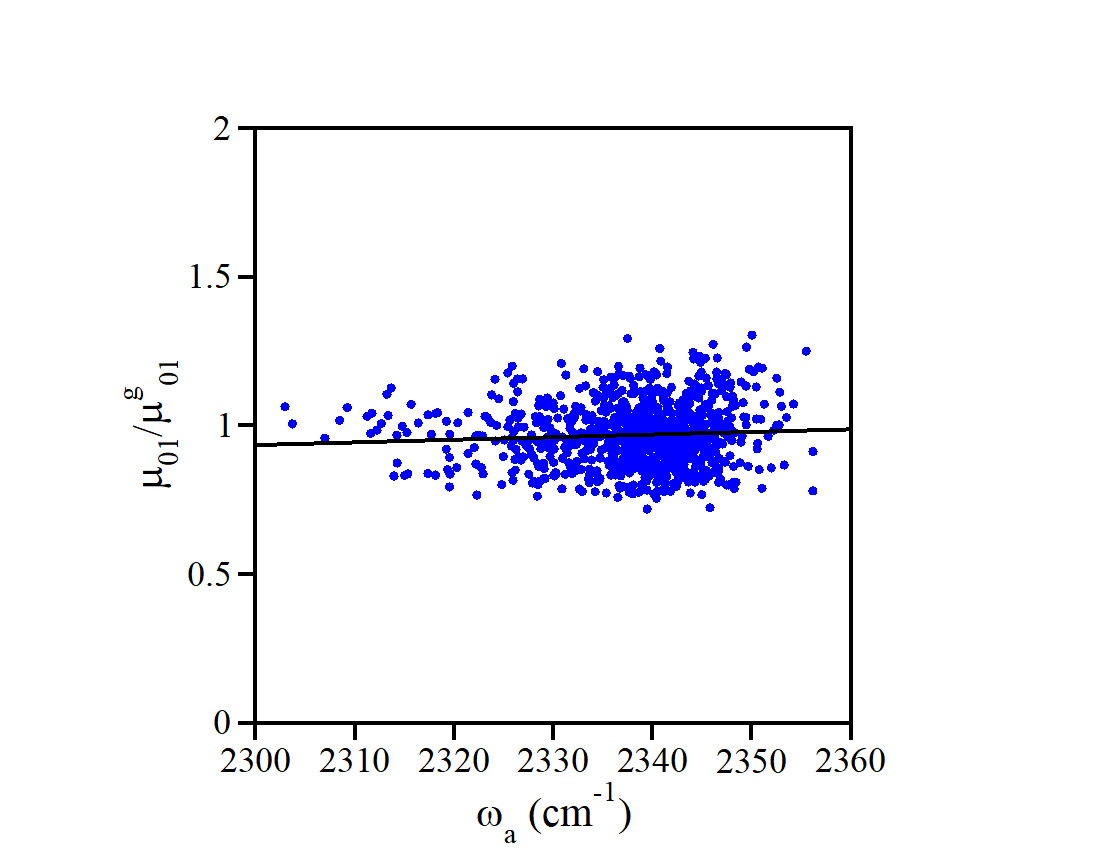
\includegraphics[width=\textwidth]{paper_03/figure3.png}
  \caption[Correlation between \(\mu_{01}\) and \(\tilde{\nu}_{3}\)]{Transition dipole moment integral, \(\mu_{01}\), of the asymmetric stretch of \ce{CO2} in 1000 \ce{CO2}-\ce{[C4C1im][PF6]} clusters versus the asymmetric stretch vibrational frequency, \(\omega_{a}\), where \(\mu_{01}^{g}\) is the transition dipole moment integral of the asymmetric stretch of \ce{CO2} in the gas-phase (blue circles). A linear fit of the data (black line) has a slope close to zero indicating that the Condon approximation is reasonable for the asymmetric stretch of \ce{CO2} in the \ce{[C4C1im][PF6]} IL.}
  \label{paper_03:fig3}
\end{figure}

A map for the solvent effects on the asymmetric \ce{CO2} vibrational frequency was constructed assuming the following form,
\begin{equation}
  \label{paper_03:eq:3}
  \Delta\omega_{\text{solvent}} = b_{1}E_{\ce{O}}^{\text{Cation}} + b_{2}E_{\ce{O}}^{\text{Anion}} + c_{1}U_{\ce{O}} + c_{2}U_{\ce{C}}
\end{equation}
where \(E\) and \(U\) represent contributions from the electric field and Lennard-Jones (LJ) interactions with the solvent, respectively. The subscript, \ce{C} or \ce{O}, indicates whether the interaction is computed at the location of the \ce{CO2} central carbon or at the oxygen atoms. For \(E_{\ce{O}}\) and \(U_{\ce{O}}\), the value used in Eq.~(\ref{paper_03:eq:3}) is the average for the two \ce{CO2} oxygen sites. The LJ interaction is computed using the expression,
\begin{equation}
  \label{paper_03:eq:4}
  U = \ \sum_{j}^{}\varepsilon_{j}\left\lbrack \left( \frac{\sigma_{j}}{r_{j}} \right)^{12} - \left( \frac{\sigma_{j}}{r_{j}} \right)^{6} \right\rbrack
\end{equation}
where the sum is over all atoms in the surrounding liquid, \(\varepsilon_{j}\) and \(\sigma_{j}\) are the LJ parameters for the atom, and \(r_{j}\) is the distance to the atom. The electric fields are calculated with respect to the oxygen atoms of \ce{CO2} and are projected along the relevant \ce{CO} bond,
\begin{equation}
  \label{paper_03:eq:5}
  E = {\hat{r}}_{\ce{CO}} \cdot \sum_{j}^{}\frac{q_{j}{\hat{r}}_{j}}{r_{j}^{2}}
\end{equation}
where the sum is over all relevant atoms in in the surrounding liquid (i.e. those associated with the cations for \(E_{\ce{O}}^{\text{Cation}}\) and those associated with the anions for \(E_{\ce{O}}^{\text{Anion}}\)), \(q_{j}\) is the partial atomic charge, \(r_{j}\) is the distance to the charge, \({\hat{r}}_{j}\) is a unit-vector directed toward the site of the charge, and \({\hat{r}}_{\mathrm{\text{CO}}}\) is a unit vector from the carbon atom of \ce{CO2} to the relevant oxygen atom. Long range electrostatics are corrected using the damped shifted force method.\cite{fennell_is_2006}

The four parameters, \(b_{1}\), \(b_{2}\), \(c_{1}\), and \(c_{2}\), in Eq.~(\ref{paper_03:eq:3}) were determined empirically by applying multiple linear regression using the \num{500} calculated frequencies in the training set (Table~\ref{paper_03:tab1}). The quality of the fit was evaluated using the \num{500} different frequencies contained in the test set (Figure~\ref{paper_03:fig2}). The root-mean-square (RMS) deviation between the test set frequencies and those predicted by Eq.~(\ref{paper_03:eq:3}) was \SI{2.7}{\wavenumber}, and the value of correlation coefficient for the fit was \(R = 0.94\). By both metrics, the quality of the spectroscopic map for predicting the \ce{CO2} asymmetric stretch vibrational frequencies in the \ce{[C4C1im][PF6]} IL is as good or better than previously published maps for other vibrational reporters in conventional solvents. Additionally, when \num{500} rigid \ce{CO2} snapshots are used as the test set, the same level of accuracy is obtained.

\begin{table}
  \centering
  \caption[Parameters of the \ce{CO2} \(\nu_{3}\) spectroscopic map]{Parameters of the spectroscopic map for the \ce{CO2} asymmetric stretch frequency in \ce{[C4C1im][PF6]}.  This map predicts the \ce{CO2} with a regression coefficient \(R = 0.94\) and a root mean squared error of \SI{2.7}{\wavenumber}. The average shift, \(\Braket{\Delta\omega}\), and standard deviation, \(\sigma(\Delta\omega)\), are reported for each term in the map.}
  \label{paper_03:tab1}
  \begin{tabular}{cccc}
    \toprule
    & & \(\Braket{\Delta\omega}\) (\si{\wavenumber}) & \(\sigma(\Delta\omega)\) (\si{\wavenumber})\\
    \midrule
    \(\omega_{g}\) & \SI{2349.1}{\wavenumber} & 0.0 & 0.0 \\
    \(a\) & \SI{-1160.9}{\wavenumber} & -6.6 & 7.0 \\
    \(b_1\) & \SI{64.4}{\wavenumber\per\au} & -0.1 & 0.4 \\
    \(b_2\) & \SI{93.2}{\wavenumber\per\au} & -1.8 & 0.7 \\
    \(c_1\) & \SI{4.70}{\wavenumber\per\kcal\mole} & -9.5 & 2.0 \\
    \(c_2\) & \SI{-3.55}{\wavenumber\per\kcal\mole} & 7.3 & 2.1 \\
    \bottomrule
  \end{tabular}
\end{table}

\begin{figure}
  \centering
  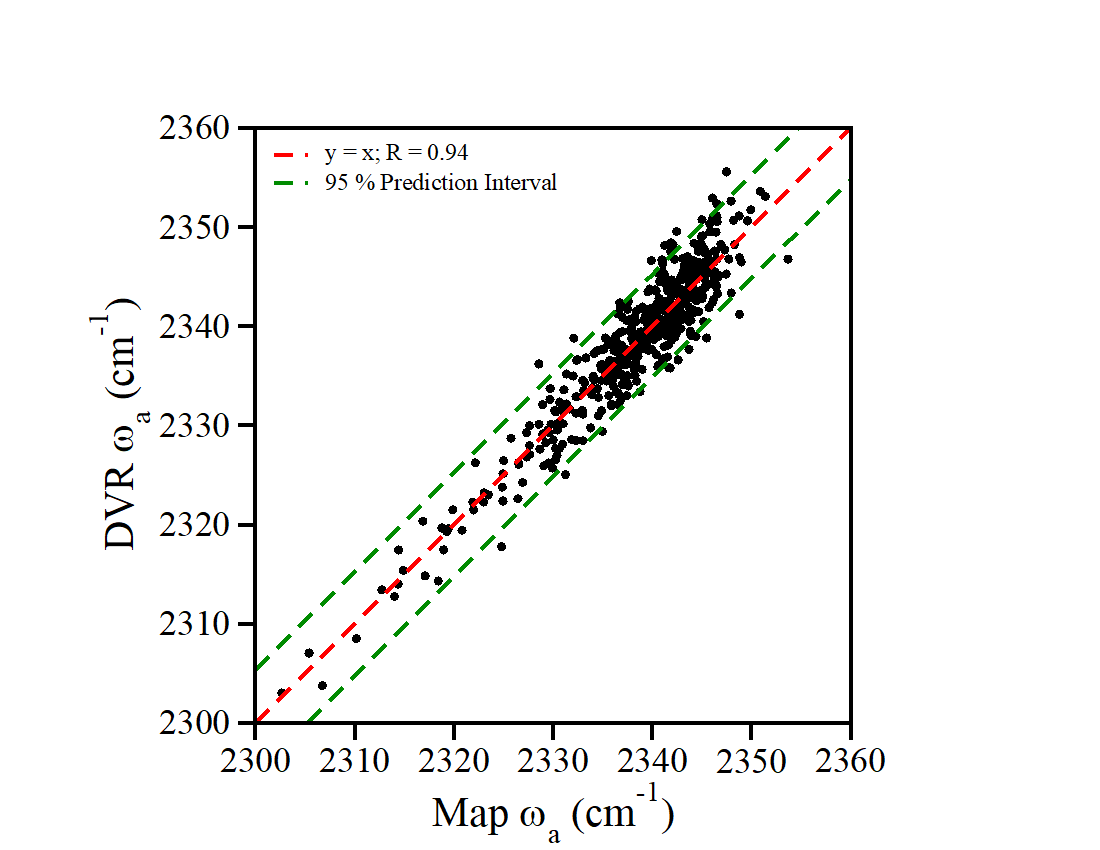
\includegraphics[width=\textwidth]{paper_03/figure2.png}
  \caption[Spectroscopic map comparison with DVR]{Relationship between \ce{CO2} asymmetric stretch frequencies in the \ce{[C4C1im][PF6]} IL calculated using the DVR method and those calculated using the spectroscopic map for the 500 test set clusters (black circles). The red line represents a perfect correlation and the 95\% prediction interval is indicated with green lines. The spectroscopic map has a regression coefficient of \(R = 0.94\) and a root means squared error of \SI{2.7}{\wavenumber}.}
  \label{paper_03:fig2}
\end{figure}

The Condon approximation, that the magnitude of the transition dipole moment is independent of the vibrational frequency of a mode, fails for some solutes that interact in a strong local way with their environment. The most important example is the \ce{OH} stretch of liquid water. The hydrogen bonds in water polarize the OH bond, increasing the oscillator strength on the red side of the vibrational band, which has a significant effect on the IR absorption line shape.\cite{corcelliJPCA-05,schmidt_pronounced_2005-1,loparoCP-07} Similar to the hydrogen bonding of water, the strong local interactions of \ce{CO2} with the ionic liquid anion could, in principle, cause the Condon approximation to fail. However, we find that the Condon approximation for the main band is adequate (Figure~\ref{paper_03:fig3}). We calculated the transition dipole moment integral, \(\mu_{01}\), of the asymmetric stretch of \ce{CO2} in \num{1000} \ce{CO2}-\ce{[C4C1im][PF6]} clusters. The details of the transition dipole moment integral calculations are provided in the Supporting Information (SI). A plot of \(\mu_{01}\) scaled by \(\mu_{01}^{g}\), the transition dipole moment integral of the asymmetric stretch of \ce{CO2} in the gas-phase, versus the asymmetric stretch vibrational frequency, \(\omega_{a}\), has a slope close to zero. This confirms that it is reasonable to regard the transition dipole as a constant factor that scales the intensity of linear and non-linear spectra but does not modify their shapes. As a result, we do not treat the environmental dependence of the transition dipole moment in our spectroscopic map; we need only treat the vibrational frequencies.

\section{\texorpdfstring{\caps{Physical Interpretation of the Spectroscopic Map}}{Physical Interpretation of the Spectroscopic Map}}
\label{paper_03:sec:IV}

The average contribution to the \ce{CO2} asymmetric stretch vibrational frequency from each of the map components is listed in Table~\ref{paper_03:tab2}. This data demonstrates that the Lennard-Jones potential energy is an important predictor of the vibrational frequency of \ce{CO2} solvated in \ce{[C4C1im][PF6]}, while the electrostatic potential plays a secondary role. This contrasts many prior spectroscopic maps where solvatochromic frequency shifts were based purely on the electrostatics of the environment.\cite{lin_water_2009-1,ohJCP-08,Miller2009} This finding is perhaps surprising at first, because one might expect electrostatics to dominate the interactions of a solute with charged solvent molecules; however, one has to consider that (1) \ce{CO2} is not dipolar or charged, and as such will not interact with uniform electric fields very strongly, and (2) the ionic liquid, particularly the \ce{[C4C1im]+} butyl tails, have large domains where the dominant interactions are dispersive. These points make it conceivable that van der Waals effects dominate the \ce{CO2}-IL interaction.

\begin{table}
  \centering
  \caption[Decomposition of the spectroscopic map LJ component]{Decomposition of the average LJ contribution to the spectroscopic map for the \ce{CO2} asymmetric stretch frequency in \ce{[C4C1im][PF6]} into attractive and repulsive components.}
  \label{paper_03:tab2}
  \begin{tabular}[]{ccc}
    \toprule
    LJ Component & Site & \(\Braket{\Delta\omega}\) (\si{\wavenumber}) \\
    \midrule
    Attractive & O & -21.7 \\
    & C & 14.8 \\
    & Sum & -6.9 \\
    Repulsive & O & 12.3 \\
    & C & -7.4 \\
    & Sum & 4.9 \\
    Total & O & -9.4 \\
    & C & 7.3 \\
    & Sum & -2.1 \\
    \bottomrule
  \end{tabular}
\end{table}

To further unravel the origin of the impact of \ce{CO2}-IL interactions on the vibrational signature of \ce{CO2}, we use the fact that the LJ contributions to the spectroscopic map can be further decomposed. In particular, we separate the LJ term into its repulsive (\({\sim r}^{-12}\)) and attractive (\(\sim r^{-6}\)) contributions (Table~\ref{paper_03:tab2}). We find that the attractive and repulsive LJ terms contribute \SI{-7.0}{\wavenumber} and \SI{+4.9}{\wavenumber}, respectively, to the overall LJ vibrational shift of \SI{-2.1}{\wavenumber}. The large contribution from the repulsive LJ term is yet another surprise. To aid in identifying the physical origins of the large repulsive LJ contribution, we performed symmetry adapted perturbation theory (SAPT)\cite{Hohenstein2011} calculations that decompose the total interaction energy into physically meaningful components. This analysis should be contrasted with the empirical spectroscopic map, where a good fit implies correlation but not necessarily causation. Our SAPT calculations yield energy contributions, but it should nevertheless be possible to estimate the relative importance of different interactions for vibrational frequencies. The SAPT decomposition supports the previous discussion in that electrostatic interactions (electrostatics, induction) plus the exchange (exchange repulsion, exchange-induction) roughly cancel (total \SI{-1.3}{\kcal\per\mole}), whereas dispersive interactions dominate the interaction (total \SI{-4.7}{\kcal\per\mole} from dispersion plus exchange-dispersion). However, the SAPT data also reveals that exchange-dispersion (the repulsive dispersion part) is over an order of magnitude smaller than the attractive dispersion contribution (10.1\% of the total dispersion interaction). This result has to be contrasted with the \textasciitilde{}40\% contribution that the repulsive LJ potential makes to the vibrations. Since the repulsive LJ contribution is the dominant repulsive interaction incorporated in our model, the SAPT results suggest that the repulsive part of the LJ potential fits an agglomerate of exchange (Pauli) repulsion stemming from charge overlap (74.7\% of the repulsive interactions), exchange induction (20.7\%) plus exchange dispersion (4.6\%).

It is likely that LJ components will be an important component of a spectroscopic map for any neutral and nonpolar solute, or any solvent where dispersive interactions, quantum effects (Pauli exchange, for instance), or higher order electrostatic interactions are particularly important. In our case, it seems logical that a higher potential at the carbon would increase the optimal length of the CO bonds, thus decreasing the local mode and normal mode frequencies. Meanwhile, at the oxygen, a larger potential would generally shorten the bond, increasing the frequency. A similar finding was observed by Brinzer \emph{et al}.\cite{Brinzer2015} However, these components only allow the \ce{CO2} vibration to respond to local effects \textemdash{} the electric field components allow it to respond to longer-range interactions. As in prior works for different solvents and solutes, the coefficients for the two electric field components are different from each other, in this case by a substantial margin. It has been previously established that \ce{CO2} interacts with the anions more strongly than with the cations in an ionic liquid.\cite{Cadena2004,akiJPCB-04,anthonyJPCB-05,Muldoon2007a,houIECR-07,ramdinIECR-12} This is reflected in the magnitude of the coefficients related to the two components, and in their average frequency contribution (Tables~\ref{paper_03:tab1}~and~\ref{paper_03:tab2}). In particular, \ce{CO2} is a Lewis acid and should generally interact with negatively charged moieties differently from positively charged ones.

\section{\texorpdfstring{\caps{Validation}}{Validation}}
\label{paper_03:sec:V}

\subsection{Experimental Frequency Distribution}
\label{paper_03:ssec:V-A}

In order to compare our calculated distributions of \ce{CO2} vibrational frequencies with experiment, we must account for the effects that broaden or narrow the IR absorption line shape beyond the underlying distribution of frequencies. The finite population lifetime of the asymmetric stretch vibration, reorientation of the \ce{CO2} molecule, and a variety of other effects can broaden the absorption spectrum. On the other hand, fast dynamics can narrow the absorption spectrum (i.e. motional narrowing). A faithful comparison to experiment requires a deconvolution of these contributions to estimate the range of instantaneous frequencies experienced by \ce{CO2}.

2D-IR spectra contain sufficient information to recover the distribution of frequencies, which would be difficult to extract from the linear IR absorption spectrum alone.\cite{Brinzer2015} Within the Kubo multi-exponential ansatz, the width of the frequency distribution is determined by the frequency fluctuation correlation function
\begin{equation}
  \label{paper_03:eq:6}
  \Braket{\delta\omega(t)\delta\omega(0)} = \sum_{i}^{N} \Delta_{i}^{2}\exp\left( - \frac{t}{\tau_{i}} \right)
\end{equation}
where \(\Delta_{i}^{2}\) are the variances of frequency modulations, and \(\tau_{i}\) are the timescales for the respective frequency fluctuations. The width of the frequency distribution is the sum of squares of the different broadening processes
\begin{equation}
  \label{paper_03:eq:7}
  \Braket{\delta\omega^{2}} = \sum_{i}^{N} \Delta_{i}^{2}
\end{equation}
The contribution of homogeneous processes whose frequency fluctuations are too fast to be resolved (specifically when \(\Delta_{i}\tau_{i} \ll 1\)) can be approximated as \(\delta(t)\Delta_{H}^{2}\tau_{H}\), which results in a frequency correlation function:
\begin{equation}
  \label{paper_03:eq:8}
  \Braket{\delta\omega(t)\delta\omega(0)} = \delta(t)\Delta_{H}^{2}\tau_{H} + \sum_{i}^{N - 1}{\Delta_{i}^{2}\exp\left( - \frac{t}{\tau_{i}} \right)} = \frac{\delta(t)}{T_{2}^{*}} + \sum_{i}^{N - 1}{\Delta_{i}^{2}\exp\left( - \frac{t}{\tau_{i}} \right)}
\end{equation}
where \(T_{2}^{*} \equiv \left( \Delta_{H}^{2}\tau_{H} \right)^{- 1}\) is the pure dephasing time and \(\delta(t)\) is the Dirac delta function. The pure dephasing time depends on the variance of the fast frequency fluctuations, \(\Delta_{H}^{2}\), and the correlation time for fast motions, \(\tau_{H}\), and the two parameters cannot be independently determined. Analyzing the change in shape of the 2D-IR spectra as a function of the waiting time can directly determine the magnitude of frequency modulations related to the sum of exponential decays, \(\sum_{i}^{N - 1}\Delta_{i}^{2}\), in Eq.~(\ref{paper_03:eq:8}). For \ce{CO2} in \ce{[C4C1im][PF6]} this sum is approximately \SI{2}{\wavenumber}.\cite{Brinzer2015}

Determining the magnitude of frequency modulations that give rise to the first term in Eq.~(\ref{paper_03:eq:8}) is more complicated. The pure dephasing time (\(T_{2}^{*}\)) is only one contributor to the experimentally determined dephasing time (\(T_{2}\)), which also depends on the population (\(T_{1}\)), and reorientational (\(T_{or}\)) motions of the molecule,
\begin{equation}
  \label{paper_03:eq:9}
  \frac{1}{T_{2}}\  = \frac{1}{T_{2}^{*}} + \frac{1}{2T_{1}} + \frac{1}{3T_{or}}
\end{equation}
The experimental dephasing time, \(T_{2}\), of the asymmetric stretch of \ce{CO2} in the \ce{[C4C1im][PF6]} IL is \SI{3.3}{\pico\second}.\cite{Brinzer2015} Since the experiment was performed in an all-parallel polarization, we cannot unambiguously determine the population and orientation relaxation times. We can estimate them, however, based on the rate of signal decay and the orientational correlation functions determined in a similar ionic liquid.\cite{Giammanco2016d,Giammanco2016} Estimates of \(T_{1} = \SI{20}{\pico\second}\) and \(T_{\mathrm{or}} = \SI{10}{\pico\second}\), suggest that vast majority contribution to \(T_{2}\) for \ce{CO2} in \ce{[C4C1im][PF6]} comes from pure dephasing. Population relaxation and orientational relaxation have a minor effect on the total dephasing time. We estimate a pure dephasing time of \(T_{2}^{*} = \SI{4}{\pico\second}\).

Finally, the variance of the frequency fluctuations, \(\Delta_{H}^{2}\), can be limited to a range by physical constraints on the values of \(\tau_{H}\). The lower limit on \(\tau_{H}\) is governed by the inertial motions of \ce{CO2} and its ionic liquid solvent shells. The timescale of the inertial response in liquid water is in the sub-\SI{60}{\femto\second} range, while that of acetonitrile is \SI{70}{\femto\second}.\cite{feckoSci-03,stengerPRL-01,Rosenthal1991} Using \SI{70}{\femto\second} as a lower limit for \(\tau_{H}\) places an upper limit on \(\Delta_{H}\) of \SI{9.7}{\wavenumber}. Fits to analytical response functions suggests that \(\Delta_{H}\ \tau_{H} \approx 0.2\) is a reasonable estimate of the dynamics that can be resolved using global fitting of the experimental data, which gives an upper limit on \(\tau_{H}\) of \SI{200}{\femto\second}, with a corresponding lower limit on \(\Delta_{H}\) of \SI{6}{\wavenumber}. Our estimate for the homogeneous width is thus, \(6 < \Delta_{H} < \SI{10}{\wavenumber}\). Combining the broadening due to fast and slow motions, the experimentally estimated total frequency width for \ce{CO2} in \ce{[C4C1im][PF6]} is between \SIrange{6.3}{10.2}{\wavenumber} (Figure~\ref{paper_03:fig4}).

\begin{figure}
  \centering
  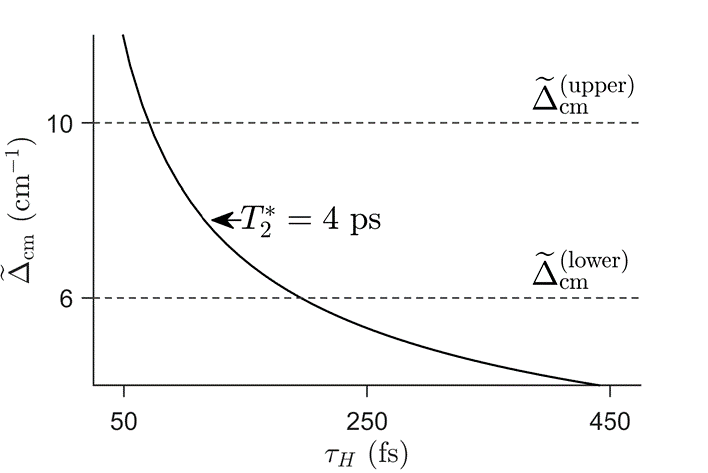
\includegraphics[width=\textwidth]{paper_03/figure4.png}
  \caption[Linewidth dependence on correlation time for fast motions]{Homogeneous instantaneous linewidth as a function of correlation time for fast motions, with \(T_{2}^{*} = \SI{4}{\pico\second}\), with upper and lower bounds estimated for \({\widetilde{\Delta}}_{H}\). The upper bound, based on an estimated fastest allowed inertial response timescale, and the lower bound, based on a threshold value of \(\Delta_{H}\tau_{H}\), are indicated by dashed horizontal lines. The resulting instantaneous frequency range for homogeneous motions is between \SIrange{6}{10}{\wavenumber}.}
  \label{paper_03:fig4}
\end{figure}

\subsection{Calculated Frequency Distributions}
\label{paper_03:ssec:V-B}

\begin{figure}
  \centering
  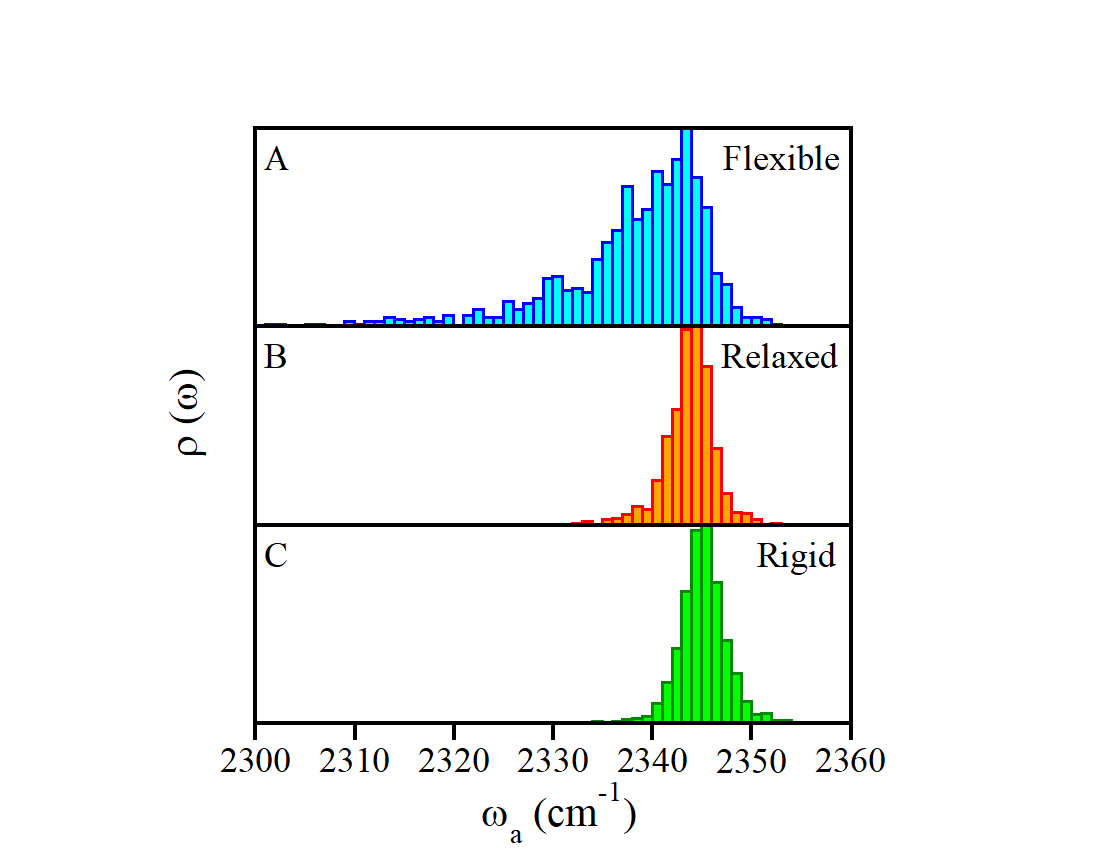
\includegraphics[width=\textwidth]{paper_03/figure5.png}
  \caption[Histograms of \ce{CO2} \(\tilde{\nu}_{3}\) from MD simulations]{Histograms of the \ce{CO2} asymmetric stretch vibrational frequency, \(\omega_{a}\), for \num{1000} \ce{CO2}-\ce{[C4C1im][PF6]} clusters. (a) Clusters extracted from an MD simulation of flexible \ce{CO2} in the \ce{[C4C1im][PF6]} IL. (b) Clusters extracted from an MD simulation of flexible \ce{CO2} in the \ce{[C4C1im][PF6]} IL, but where the \ce{CO2} geometry is relaxed. (c) Clusters extracted from an MD simulation of rigid \ce{CO2} in the \ce{[C4C1im][PF6]} IL.}
  \label{paper_03:fig5}
\end{figure}

Figure~\ref{paper_03:fig5}a shows the distribution of \ce{CO2} asymmetric stretch vibrational frequencies computed using the spectroscopic map for 1000 statistically independent snapshots collected from an MD simulation of flexible \ce{CO2} in \ce{[C4C1im][PF6]}. These are the same snapshots that were used to parametrize and validate the spectroscopic map in Section III. The distribution is peaked at approximately \SI{2344}{\wavenumber} and its standard deviation is \SI{7.4}{\wavenumber}. Both of these values are in reasonable agreement with experiment (\SI{2342.5}{\wavenumber} and \SIrange{6.3}{10.2}{\wavenumber}). Qualitatively, the distribution exhibits a significant asymmetry with a mean frequency of \SI{2339.9}{\wavenumber} that is about \SI{4}{\wavenumber} to the red of the peak frequency. The experimental IR absorption line shape, however, does not show signs of such asymmetry in the underlying distribution of frequencies.

The source of the asymmetry in the distribution of frequencies in Figure~\ref{paper_03:fig5}a is the contribution to the spectroscopic map from the \ce{CO2} bend angle, Eq.~(\ref{paper_03:eq:2}). This is illustrated in Figure~\ref{paper_03:fig5}c, where we have calculated the distribution of \ce{CO2} asymmetric stretch vibrational frequencies for 1000 statistically independent snapshots collected from an MD simulation of rigid \ce{CO2} in \ce{[C4C1im][PF6]}. Since the \ce{CO2} molecule has an angle of \ang{180} in each of the snapshots, the contribution to the calculated vibrational frequency from the \ce{CO2} bend angle is zero. The resulting distribution is correctly symmetric with a mean frequency of \SI{2346.5}{\wavenumber} and a standard deviation of \SI{2.3}{\wavenumber}. The calculated distribution is centered \SI{4}{\wavenumber} to the blue of the experimental distribution, and it is narrower than the lower estimate of the experimental distribution by \SI{4}{\wavenumber}.

The results in Figure~\ref{paper_03:fig5}a~and~\ref{paper_03:fig5}c represent two extremes \textemdash{} one where the \ce{CO2} bend is treated classically (Figure~\ref{paper_03:fig5}a) and another where the \ce{CO2} bend is effectively neglected (Figure~\ref{paper_03:fig5}c). When the \ce{CO2} bend is classical, it is assumed that the \ce{CO2} asymmetric stretch vibrational frequency depends on the instantaneous value of the bend angle, Figure~\ref{paper_03:fig1} and Eq.~(\ref{paper_03:eq:2}). However, the asymmetric distribution suggests that this approach is incorrect. In fact, a simple thought experiment reinforces the problems associated with regarding the \ce{CO2} bend as a classical variable. Consider a non-rotating \ce{CO2} molecule isolated in the gas-phase. If all of the vibrations of the \ce{CO2} molecule are quantum mechanical, the distribution of each of the four vibrations is a delta function. However, if the bend is classical with a kinetic energy commensurate with room temperature, the distribution of asymmetric stretch vibrational frequencies will incorrectly have a finite width. One solution to this conundrum is to adopt a fully quantum mechanical treatment of the \ce{CO2} vibrations. This would require the construction of a four-dimensional potential energy surface for each of the 1000 benchmark \ce{CO2}-\ce{[C4C1im][PF6]} clusters, which is computationally intractable.

\begin{figure}
  \centering
  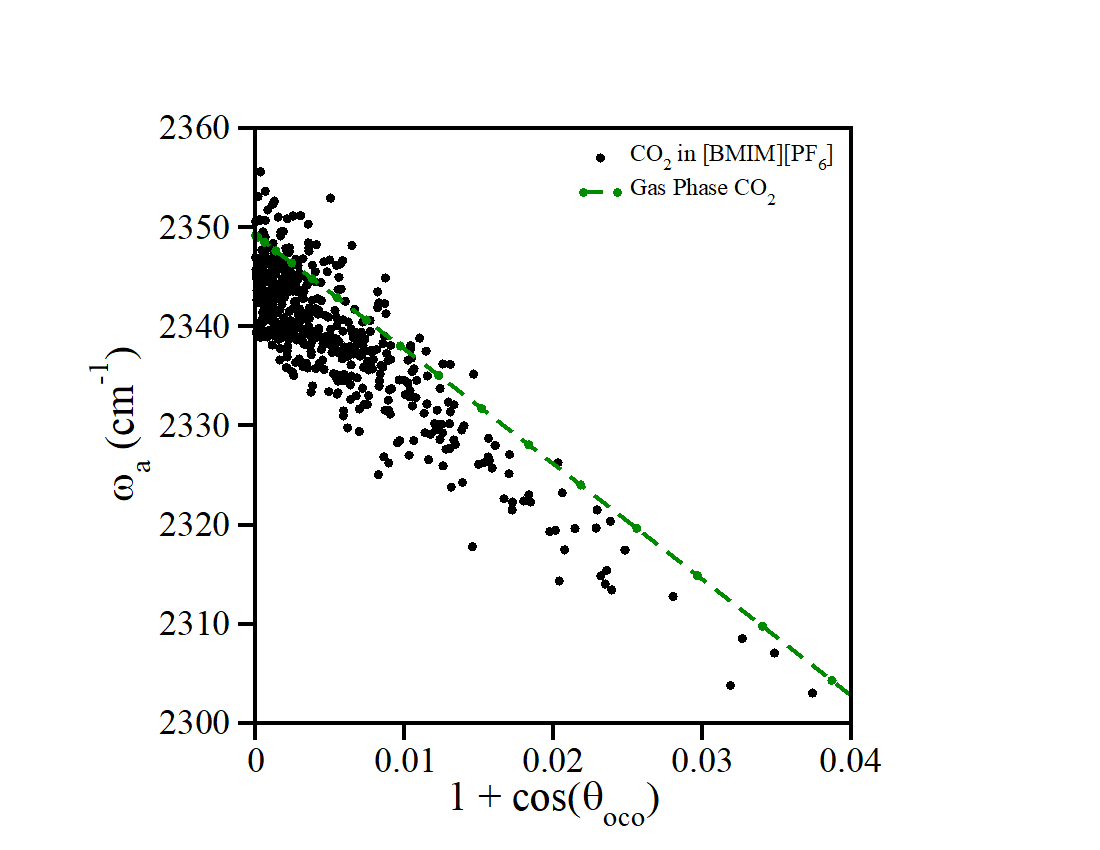
\includegraphics[width=\textwidth]{paper_03/figure1.png}
  \caption[Relationship between \ce{CO2} \(\tilde{\nu}_{3}\) and \(1 + \cos{\theta_{\ce{OCO}}}\)]{Relationship between the \ce{CO2} asymmetric stretch vibrational frequency and the \ce{OCO} angle, \(\theta_{\ce{OCO}}\), for \ce{CO2} in the gas-phase (green circles) and in the \ce{[C4C1im][PF6]} IL (black circles). The gas-phase data are perfectly correlated with \(1 + \cos{\theta_{\ce{OCO}}})\). The vibrational frequencies for \ce{CO2} in the \ce{[C4C1im][PF6]} solvent also show this relationship, but additional solvation effects on the frequency are also present.}
  \label{paper_03:fig1}
\end{figure}

An alternate strategy is to treat the influence of the \ce{CO2} bend on the asymmetric stretch vibrational frequency using first-order perturbation theory. Instead of utilizing the instantaneous \ce{CO2} angle in Eq.~(\ref{paper_03:eq:2}), \(\theta\), we would instead use the average angle, \(\Braket{\theta} = \Braket{ \varphi_{0} | \theta | \varphi_{0} }\), where \(\varphi_{0}(\theta)\) is the ground vibrational wavefunction for the \ce{CO2} bend. Returning to the \ce{CO2} in the gas-phase thought experiment, the average angle is constant and equal to 180º. Thus, there would correctly be no contribution to \ce{CO2} asymmetric stretch vibrational frequency. In contrast, the instantaneous average bend angle will fluctuate away from \ang{180} in an IL because of asymmetric solvation by the solvent. Of course, we do not have access to vibrational wavefunction for the \ce{CO2} bend for the benchmark \ce{CO2}-\ce{[C4C1im][PF6]} clusters, nor when we wanted to utilize the spectroscopic map to analyze an MD simulation. An additional approximation is necessary. If we were to regard the \ce{CO2} bend as harmonic, then the average angle is given by the instantaneous distortion of the \ce{CO2} geometry by the environment. For the benchmark clusters, the geometry distortion can be determined by optimizing the geometry of the \ce{CO2} molecule using the classical MD force field and a conjugate gradient minimization while holding fixed both the center-of-mass of the \ce{CO2}, as well as the configuration of the IL solvent. The map is then used to calculate the vibrational frequency for the relaxed snapshot.

Figure~\ref{paper_03:fig5}b shows the distribution of \ce{CO2} asymmetric stretch vibrational frequencies computed using the spectroscopic map for \num{1000} statistically independent snapshots collected from an MD simulation of flexible \ce{CO2} in \ce{[C4C1im][PF6]} where the \ce{CO2} bend angle has been relaxed. On average, the relaxed bend angle is \ang{178.4}, and the distribution of frequencies is nearly symmetric with a mean frequency of \SI{2343.8}{\wavenumber} and a standard deviation of \SI{2.4}{\wavenumber}. The mean frequency is in excellent agreement with experiment and differs by only \SI{1.3}{\wavenumber}. Note that this agreement implies that the spectroscopic map is able to accurately capture the solvatochromic shift of the \ce{CO2} asymmetric stretch vibrational frequency from the gas-phase to the \ce{[C4C1im][PF6]} IL. The width of the distribution is too narrow compared to the estimated width of the experimental distribution of \SIrange{6.3}{10.2}{\wavenumber}. There are several possible sources for the discrepancy in the width of the distribution, including inaccuracies associated with the approximate perturbative approach for the effect of the bend on the asymmetric stretch frequency. However, the overall agreement with experiment is encouraging.

It is instructive to compare the distributions in Figures~\ref{paper_03:fig5}b (relaxed \ce{CO2}) and \ref{paper_03:fig5}c (rigid \ce{CO2}). Both distributions are symmetric and they have nearly the same widths: \SI{2.4}{\wavenumber} and \SI{2.3}{\wavenumber}, respectively. Thus, within the approximate perturbative approach, the bend has very little influence on the width of the distribution. The averages of the distributions differ more significantly: \SI{2343.8}{\wavenumber} and \SI{2346.5}{\wavenumber}, respectively. The bend shifts the distribution to the red and into better agreement with experiment. Overall, the role of the bend is relatively minor resulting in a redshift of the distribution by \SI{2.7}{\wavenumber}. These results suggest several options for how the bend is treated when the map is applied in conjunction with MD simulations to understand the spectroscopy and spectral diffusion dynamics of \ce{CO2} in the \ce{[C4C1im][PF6]} IL in Paper III\cite{Brinzer2018} in this series. The simplest strategy is to hold the \ce{CO2} rigid and to shift the calculated frequencies by \SI{2.7}{\wavenumber}. In essence, this would just account for the average effect of the \ce{CO2} angle on the asymmetric stretch frequencies. A more computationally intensive strategy is a simulation with \ce{CO2} flexible, but where the geometry of the \ce{CO2} is optimized using the classical force field. The efficacy of these approaches will be evaluated in Paper III\cite{Brinzer2018}.

\section{\texorpdfstring{\caps{Conclusions}}{Conclusions}}
\label{paper_03:sec:VI}

% TODO at the minimum, this passage is missing things from the final paper!
In this paper we have developed and validated a spectroscopic map that is the foundation for a molecular interpretation of ultrafast vibrational spectroscopy of \ce{CO2} in ionic liquids. In addition, we have established important insights into the solvatochromic shift of the \ce{CO2} asymmetric stretch vibrational frequency in ILs. We analyzed the physical origin of the vibrational frequency shifts using SAPT energy decomposition schemes. Unlike other vibrational chromophores, electrostatics alone poorly predict the vibrational frequency. While the most important contributor to the electrostatic part of the spectroscopic map is the field from the anion, both attractive dispersion interactions and repulsive charge overlap forces (Pauli repulsion) play additional important roles. Finally, while the \ce{CO2} bend angle influences the asymmetric stretch frequency, we have shown that the geometry of the \ce{CO2} molecule is only slightly perturbed by the IL, so regarding the \ce{CO2} as rigid is generally sufficient to capture the structural relaxation of the IL relative to the \ce{CO2}.

\section{\texorpdfstring{\caps{Acknowledgements}}{Acknowledgements}}

The authors thank Prof. Kenneth D. Jordan for helpful discussions. SAC is grateful for financial support from the National Science Foundation (CHE-1565471), the American Chemical Society Petroleum Research Fund (52648-ND6), and the Sustainable Energy Initiative at the University of Notre Dame. SAC and CAD are also thankful for high performance computing resources and support from the Center for Research Computing at the University of Notre Dame. Computational resources were also provided by the Center for Simulation and Modeling at the University of Pittsburgh. SGR acknowledges financial support from the National Science Foundation (CHE-1454105).

\section{\texorpdfstring{\caps{Supporting Information}}{Supporting Information}}
\label{paper_03:sec:SI}

Details regarding the transition dipole moment integral calculations in Figure~\ref{paper_03:fig3}.

\subsection{Transition Dipole Moment Calculations}

The intensity of a vibrational transition, \(\tilde{\nu}_{if}\), is related to the dipole moment matrix element between the two states, \(\Braket{\vec{\mu}_{if}}\)
\begin{equation}
  \label{paper_03:eq:S1}
  I \left( \tilde{\nu}_{if} \right) = \frac{8\pi^{3}N_{A}}{3hc\left( 4\pi\epsilon_{0} \right)} \tilde{\nu}_{if} \left| \vec{\mu}_{if} \right|^{2} (N_{i} - N_{f})
\end{equation}
where \(N_{A}\) is Avogadro's number, \(N_{k}\) is the number of particles in the \(k\)th state and \(\left| \vec{\mu}_{if} \right|^{2}\) is the squared norm of the transition dipole moment (TDM) integral between the two states.\cite{Carbonniere2010} Because all values in equation~\ref{paper_03:eq:S1} are constant (at a specific temperature) vibrational intensities for particular transitions are proportional to the squared norm of the TDM vector. Thus, the central property to calculate in order to evaluate the strength of the Condon approximation is \(\Braket{\vec{\mu}_{if}}\).

We can calculate the matrix elements of the dipole moment operator in a similar fashion as the bond length matrix elements were calculated in paper 1. Before, we used the value of the bond length at each grid point as a representation of the bond length operator. Similarly, we use the \(x\), \(y\), and \(z\) components of the dipole moment at each grid point (reported by a quantum chemistry program \textemdash{} in this case, Q-Chem\cite{Shao2015} \textemdash{} as the appropriate integral over the entire charge density) as a representation of the dipole moment operator,
\begin{equation}
  \label{paper_03:eq:S2}
  \vec{\mu} = \sum_{k = 1}^{3} \mu^k \widehat{k}
\end{equation}
where \(\widehat{k}\) is the \(k^{\text{th}}\) Cartesian basis vector. The dipole moment matrix elements are, for a two dimensional grid,
\begin{equation}
  \label{paper_03:eq:S3}
  \Braket{ \vec{\mu}_{if} } = \sum_{k = 1}^{3} \sum_{l = 1}^{N} \sum_{j = 1}^{N} \psi_{jl}^{i} \mu_{jl}^{k} \widehat{k} \psi_{jl}^{f}
\end{equation}
where the \(\psi_{jl}^{n}\) are the vibrational wavefunctions for state \(n\) on grid point \((j,l)\) returned by the DVR method. We have evaluated the accuracy of this method for \ce{CO2} in two ways. First, we calculate the norm of the TDM integral for the symmetric and asymmetric stretches of \ce{CO2} in the gas phase and compare these to experiment.\cite{DOWNING197566} The results are shown in Table~\ref{paper_03:tab:S1}, and the accuracy is excellent.

Next, we evaluated the accuracy of this method for \ce{CO2} in solution. A previously used method for evaluating the Condon approximation for vibrational reporters in solution is to (1) optimize the vibrational subsystem of interest with DFT while freezing all other degrees of freedom, (2) calculate the harmonic vibrational frequency and intensity for the vibrational subsystem using the same DFT method, then (3) repeat this for many statistically independent snapshots of the reporter in solution.\cite{schmidt_pronounced_2005-1} This process was completed for \num{25} snapshots of \ce{CO2} in IL solution for the asymmetric stretch. DVR asymmetric stretch frequencies and TDMs were also calculated for the \num{25} optimized (post step 1) snapshots. In order to facilitate comparison, the square roots of the intensities were taken. The resulting values and the TDMs were divided by their respective gas phase values. These values are plotted against each other in figure~\ref{paper_03:fig:S1}. The agreement between the two methods is excellent (\(R = 0.994\)). This new method has the advantage of being essentially computationally free to perform anytime a DVR calculation has already been done. Due to the possibility of parallelization, DVR calculations can be much more computationally inexpensive than regular vibrational frequency calculations.

\begin{table}[b]
  \centering
  \caption{Transition dipole moments for gas phase stretching modes of \ce{CO2}.}
  \label{paper_03:tab:S1}
  \begin{tabular}{ccc}
    \toprule
    Mode & DVR (\si{\debye}) & Experiment (\si{\debye})\cite{DOWNING197566} \\
    \midrule
    \(\omega_{s}\) & \num{1.1e-13} & \num{0.0} \\
    \(\omega_{a}\) & \num{3.4e-1} & \num{3.3e-1} \\
    \bottomrule
  \end{tabular}
\end{table}

\begin{figure}
  \centering
  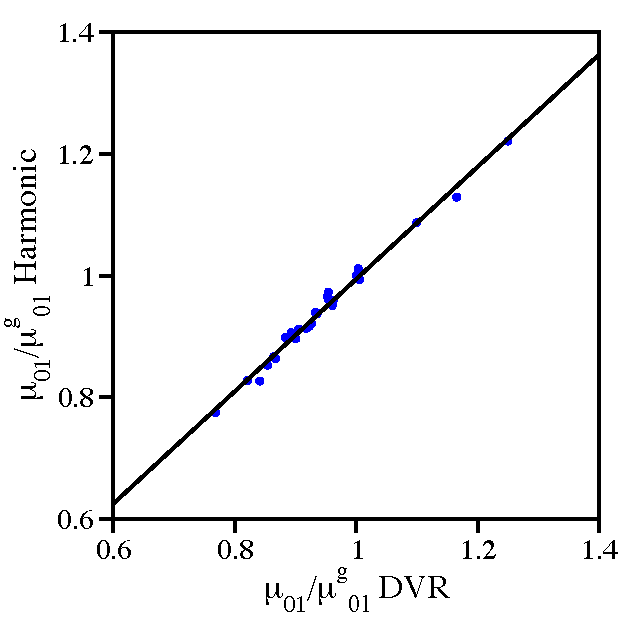
\includegraphics[width=\textwidth]{paper_03/figureS1.pdf}
  \caption{Normalized transition dipole moment for the asymmetric stretch of \ce{CO2} as calculated by a quantum chemistry program and as calculated by the DVR method (blue dots). The black line is the best fit line, \(y = 0.97x + 0.07\). The correlation coefficient is 0.994.}
  \label{paper_03:fig:S1}
\end{figure}
